\subsection{Results of \SOPT-differential \pt spectra at \tracklet 0--1\%}\label{Sec:ResSpec}

The \pt spectra for jet-like and isotropic events are presented in Figures~\ref{Fig:CombSpectraA} and~\ref{Fig:CombSpectraB} for \tracklet \topone{} together with the \SOPT unbiased reference. The trends of the spectral shapes are consistent between all observed particle species, showcasing a significant hardening (softening) of the \pt in the low (high) \SOPT selection, relative to the inclusive high-multiplicity event class, respectively. These trends are also well reflected in the model predictions. The PYTHIA 8.2 default Monash tune can describe the qualitative trends of the \SOPT selection. However, a large quantitative deviation from data is observed in the \pt differential production of light-flavor hadrons, in particular the non-strange hadrons. The PYTHIA 8.2 rope tune is able to describe the measured data for strange hadrons very well, but overestimates the total amount of produced non-strange hadrons. Similar observations can also be seen when contrasting Herwig 7.2 with EPOS-LHC, where EPOS-LHC overestimates the total yields, but is able to describe the \SOPT-differential interplay for the mesons quite well. These large deviations are well known from previous studies~\cite{13tevvsmultpapers}.

\begin{figure}[h!]
    \centering
    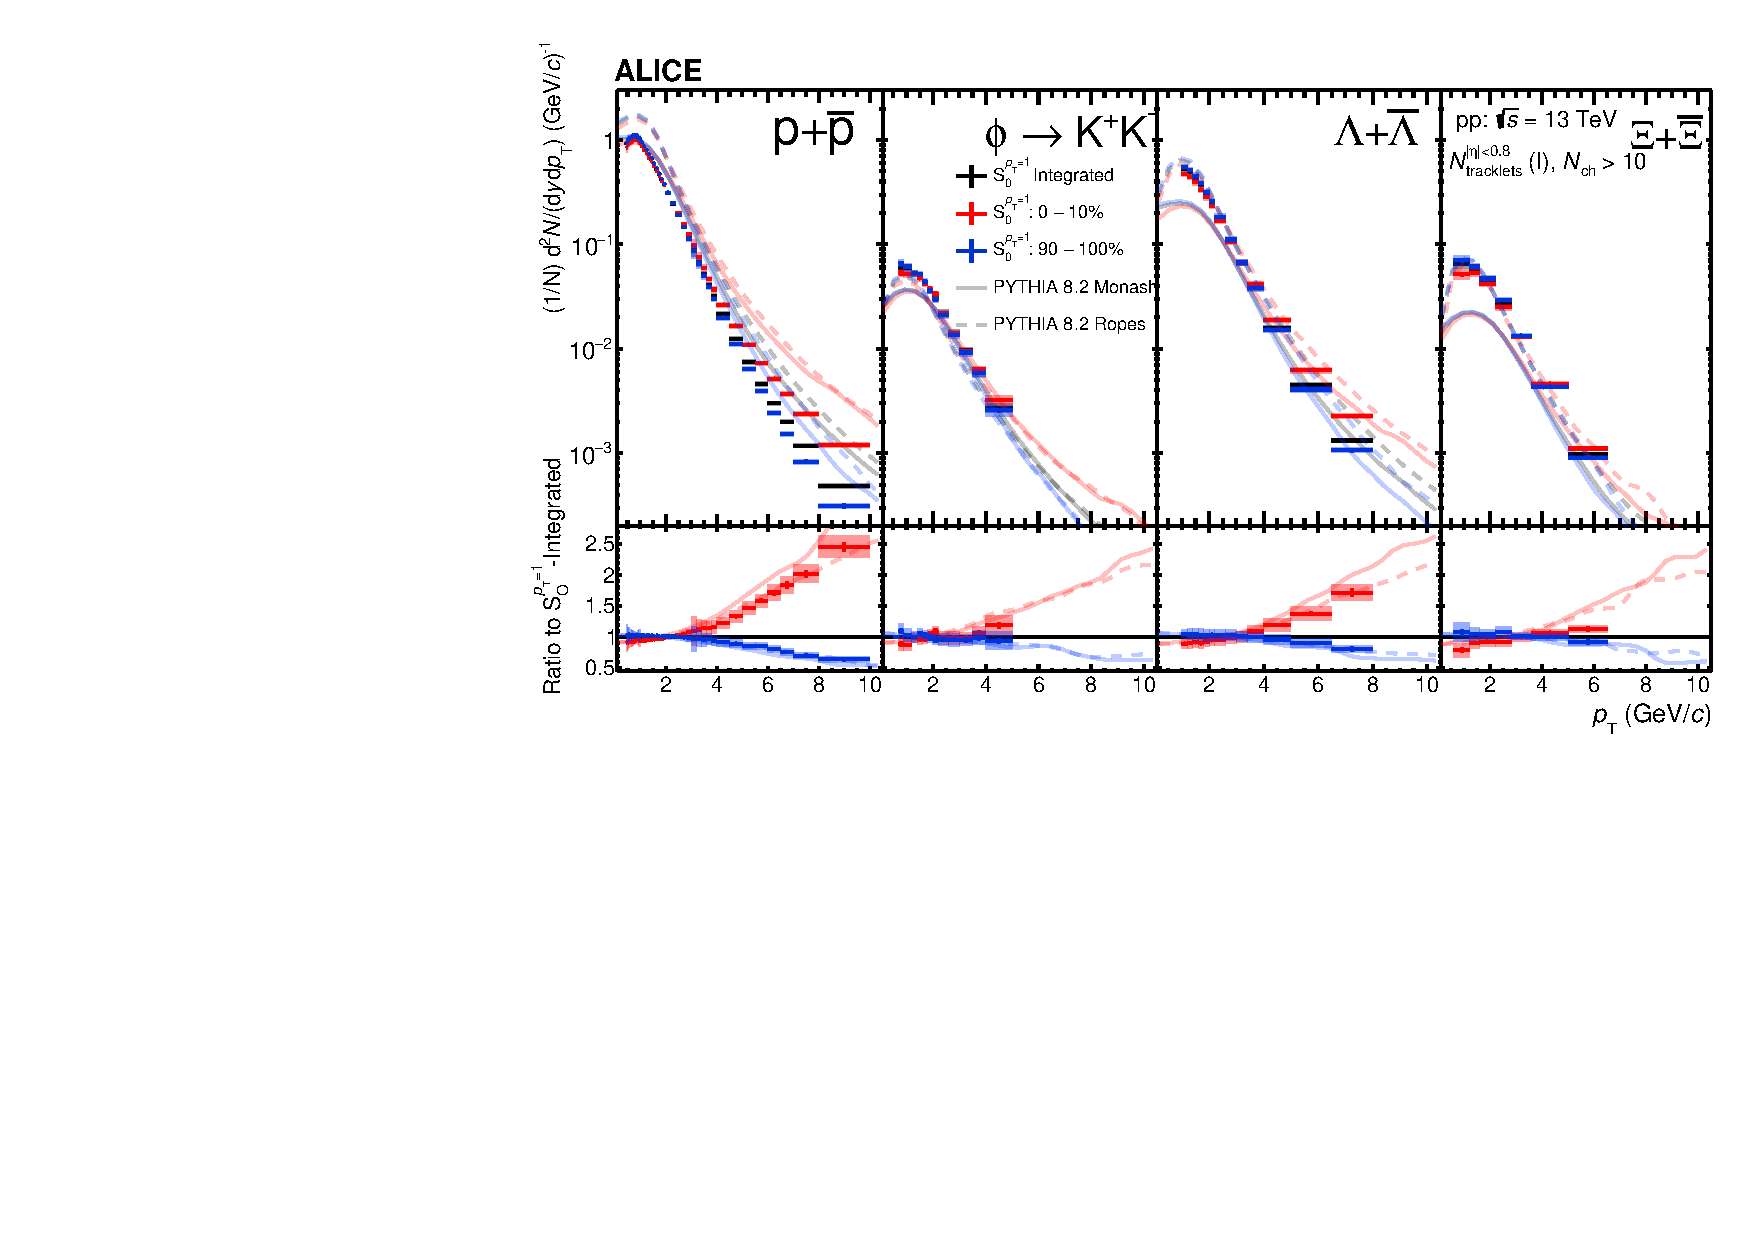
\includegraphics[scale=0.8]{figures/BaryonsSpectra_SOPT_10_NSPD_1_PY.pdf}
    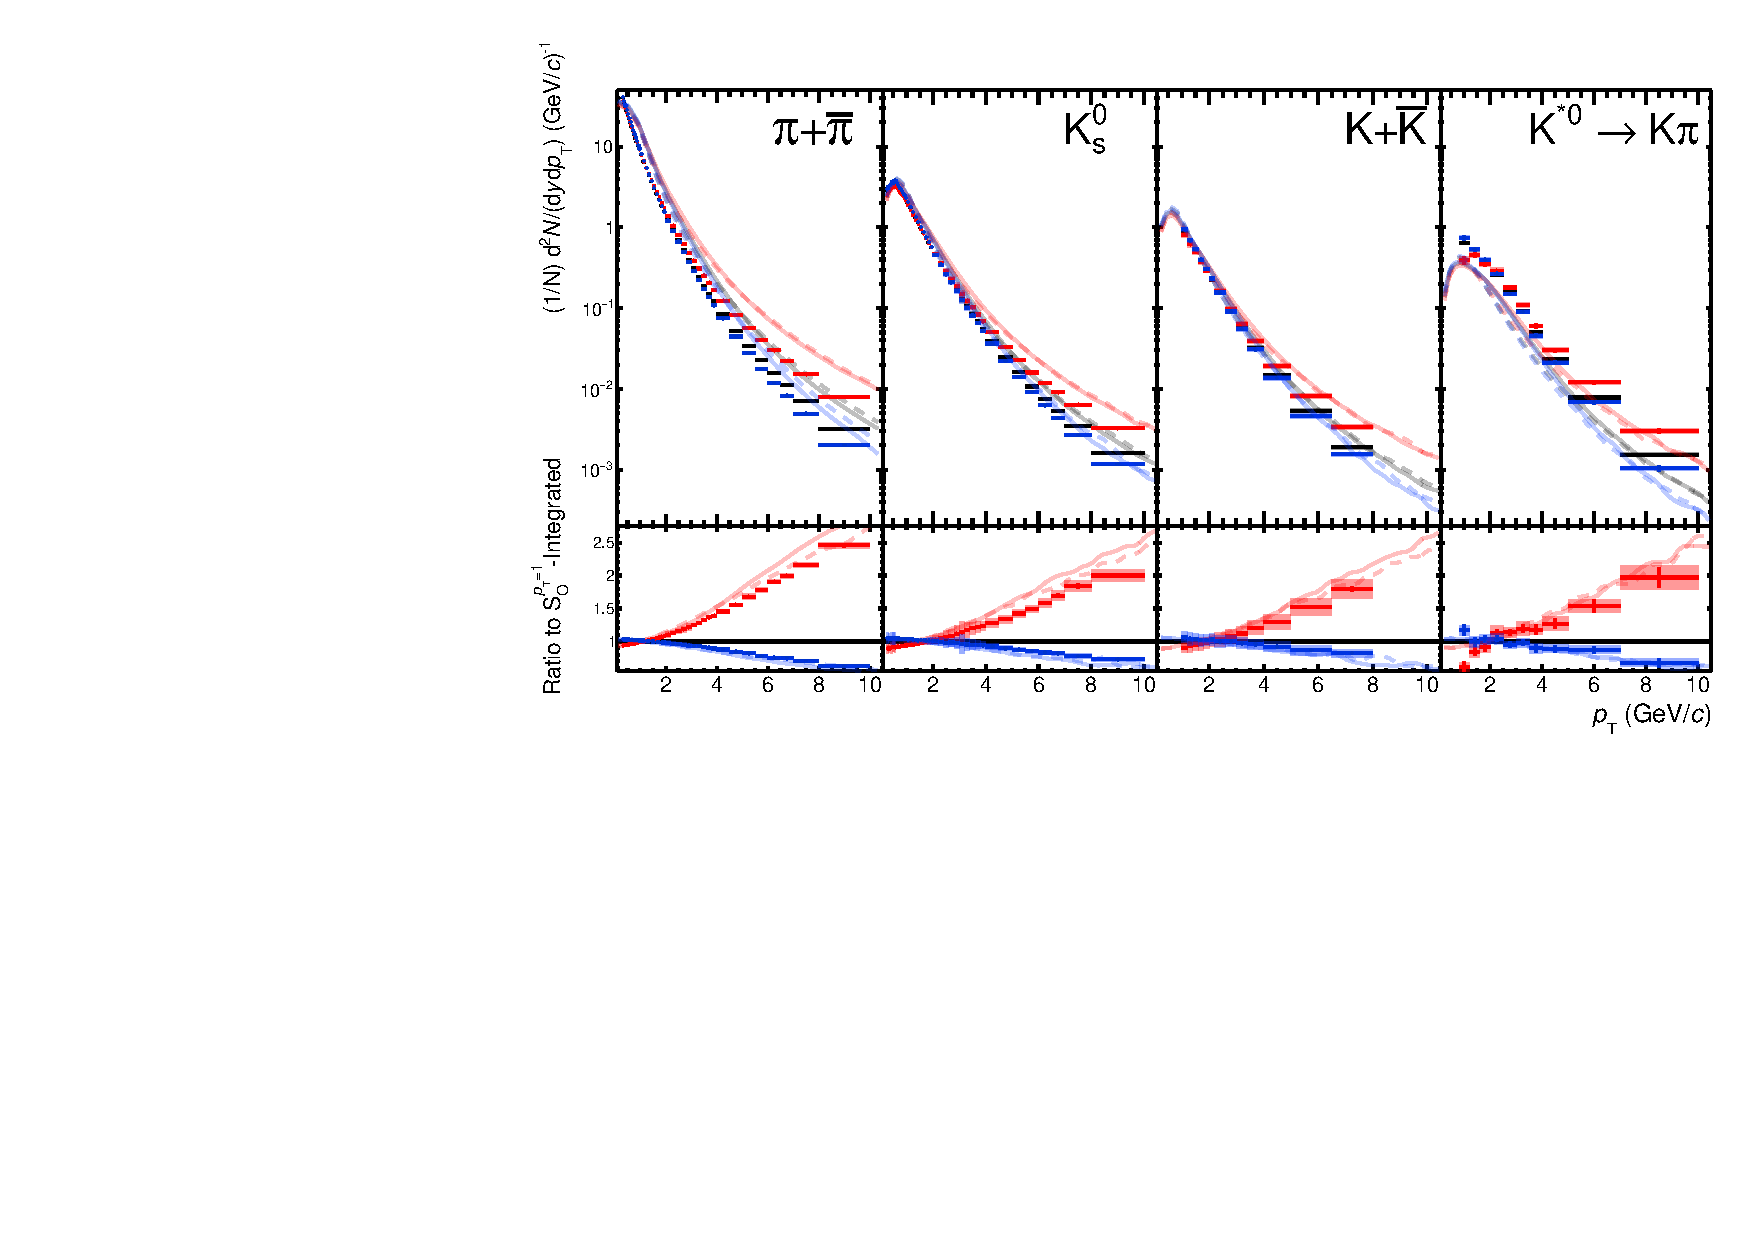
\includegraphics[scale=0.8]{figures/MesonsSpectra_SOPT_10_NSPD_1_PY.pdf}
    \caption{Transverse momentum distribution of \pikp, \KSTAR, \PHI, \KOs, \LA and \XI for \SOPT classes selected for events at high-multiplicity, determined by events in the top 1\% of \tracklet. The lower panels present the ratio between the \SOPT-integrated and \SOPT-differential events. Statistical and total systematic uncertainties are shown by error bars and boxes, respectively. The curves represent PYTHIA 8.2 model predictions of the same measurement. The average statistical uncertainties from the predictions across all particle species range in the order of 1--15 \% from low-to-high \pt.} 
    \label{Fig:CombSpectraA}
\end{figure}

\begin{figure}[h!]
    \centering
    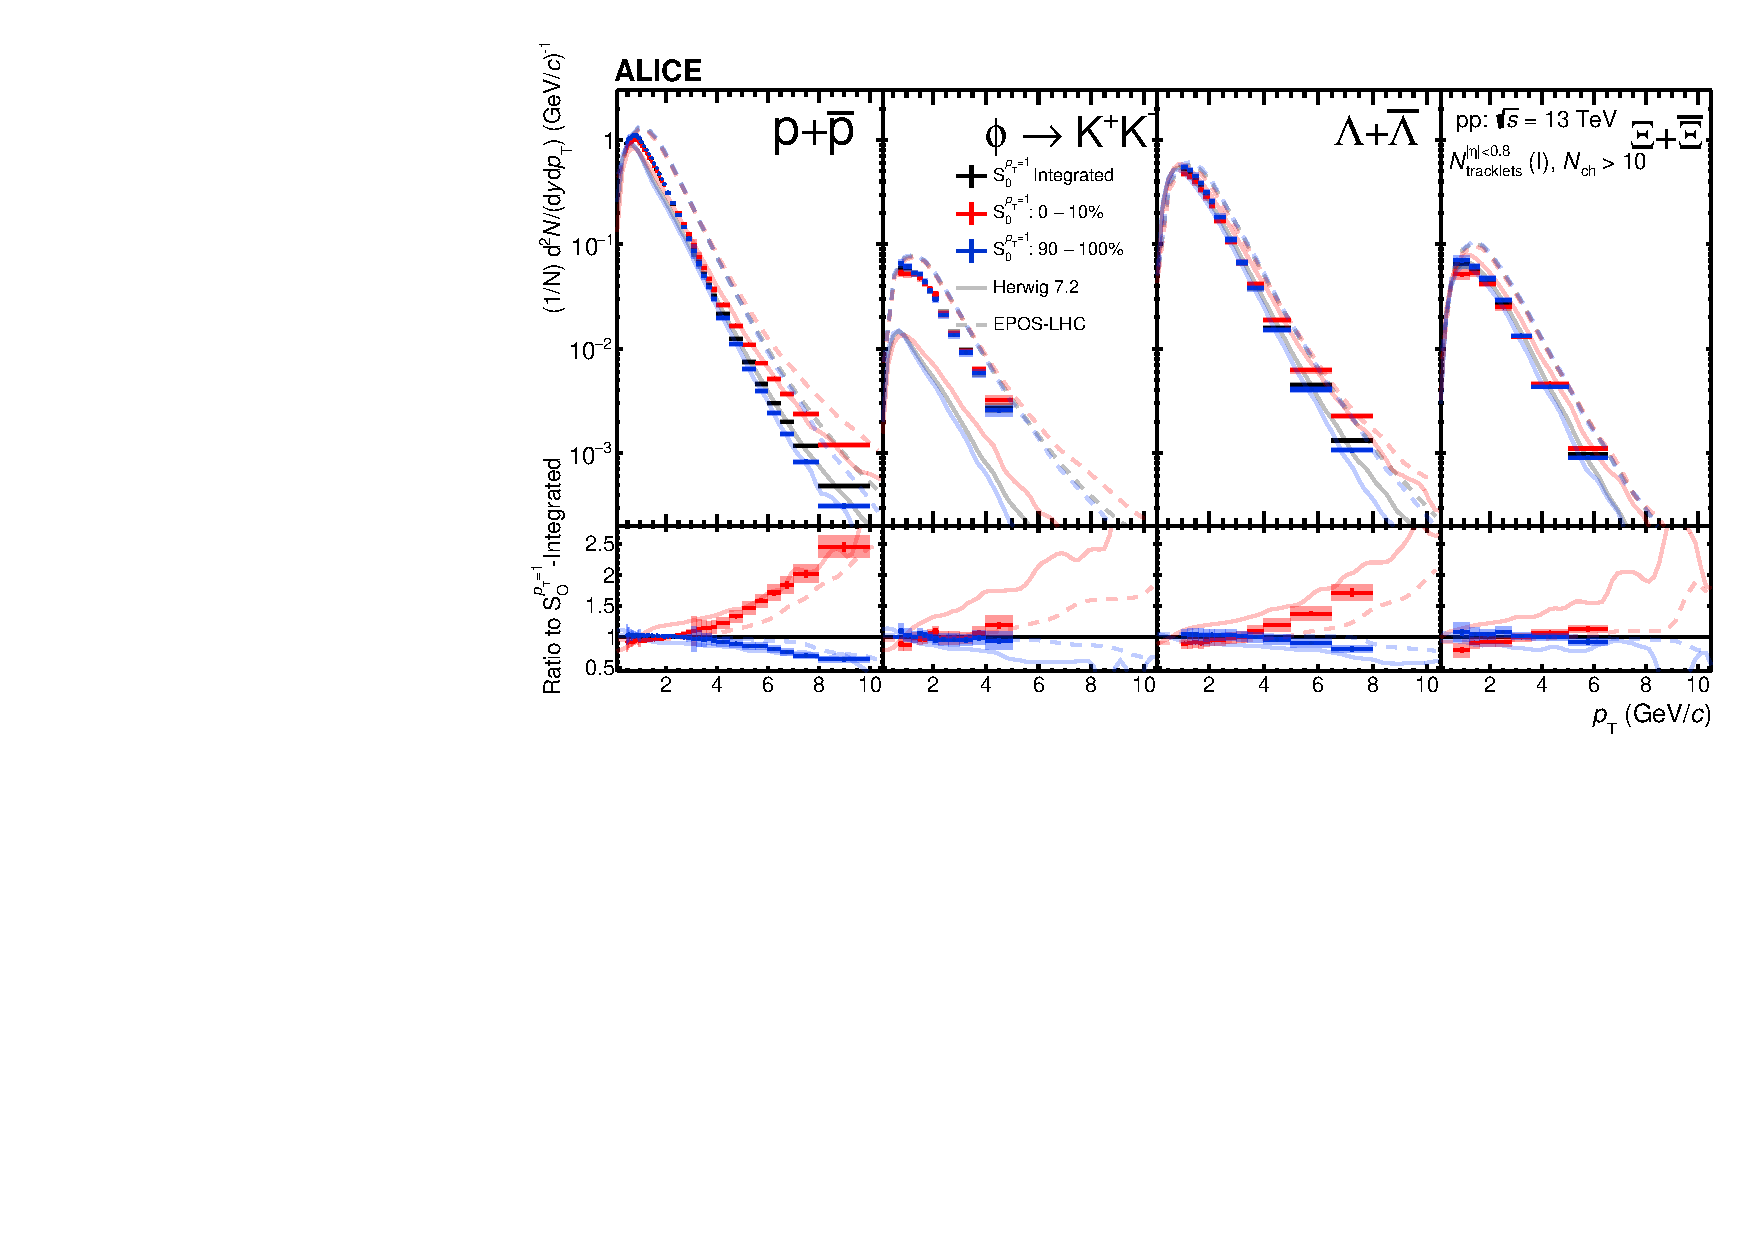
\includegraphics[scale=0.8]{figures/BaryonsSpectra_SOPT_10_NSPD_1_HW.pdf}
    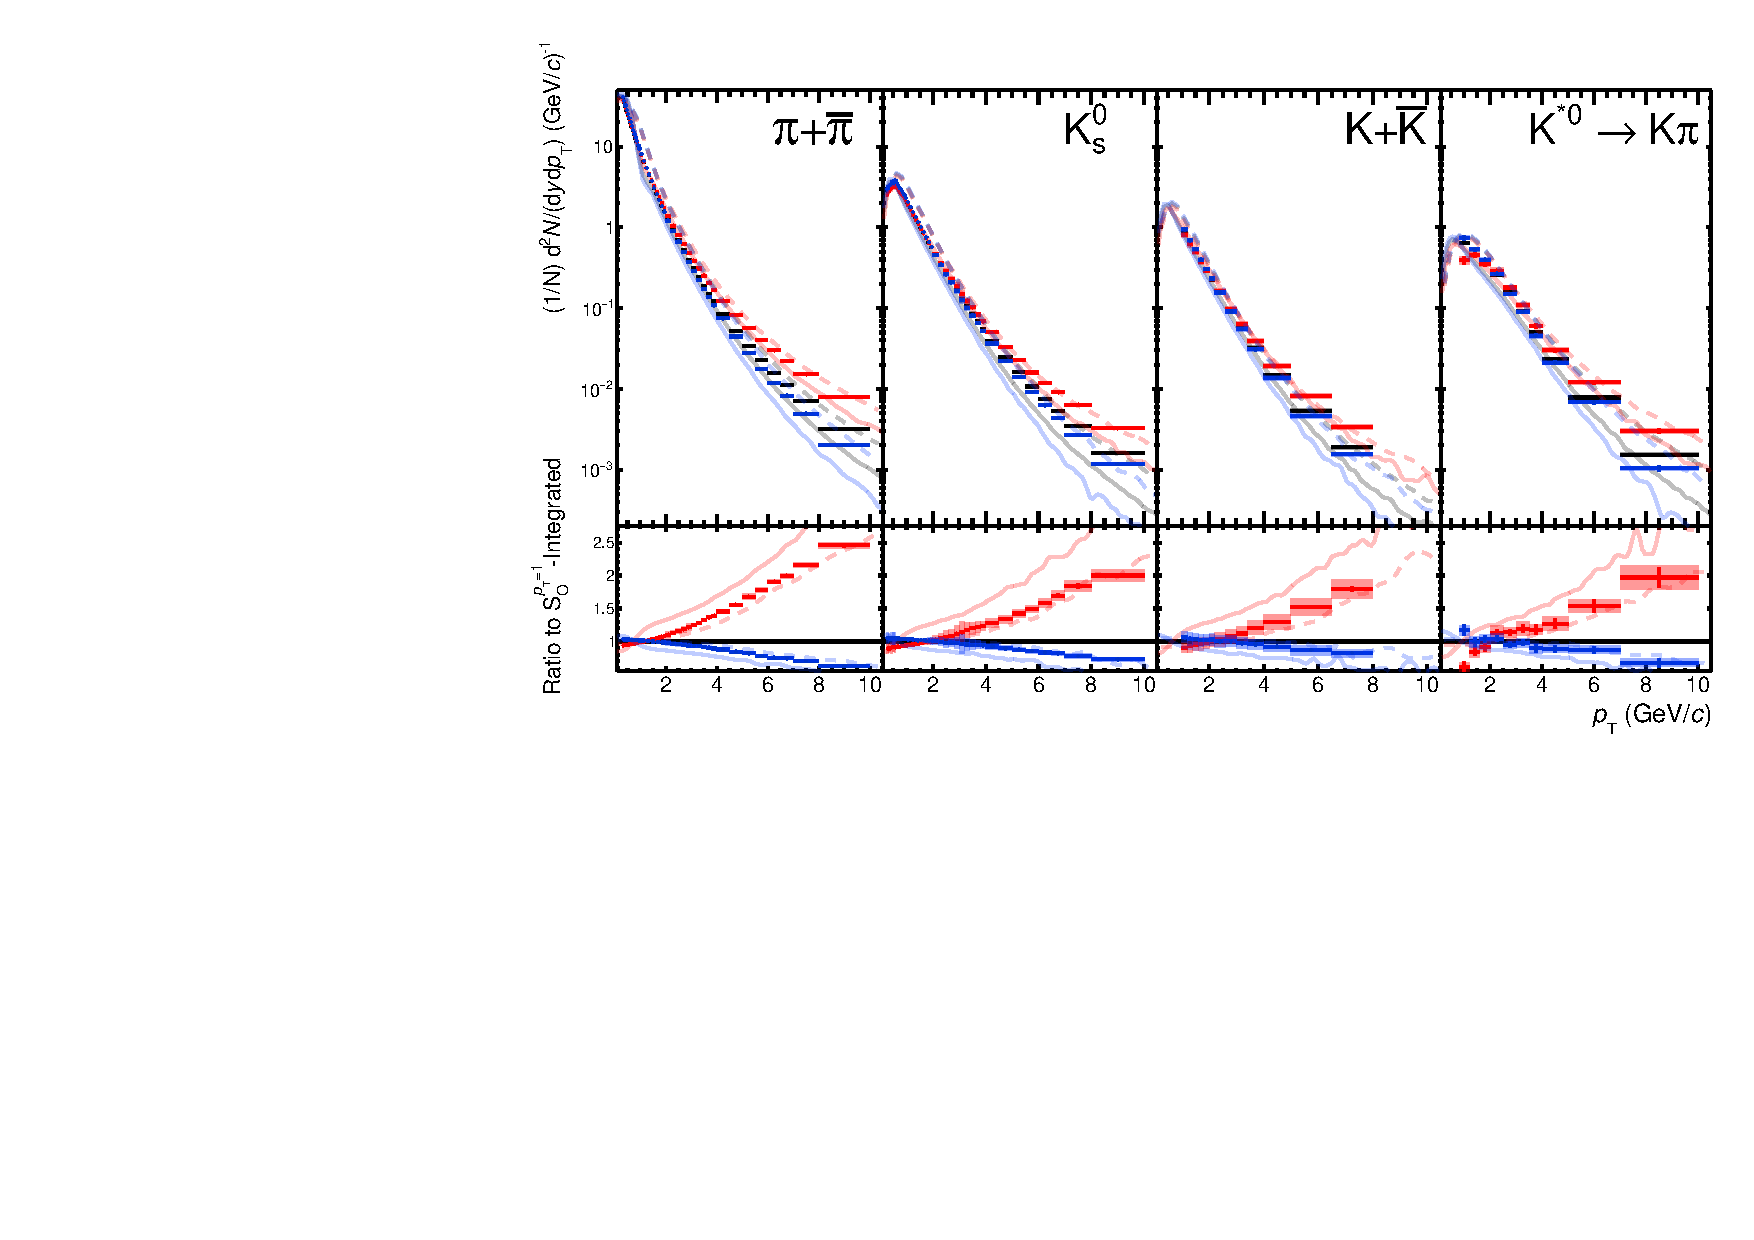
\includegraphics[scale=0.8]{figures/MesonsSpectra_SOPT_10_NSPD_1_HW.pdf}
    \caption{Transverse momentum distribution of \pikp, \KSTAR, \PHI, \KOs, \LA and \XI for \SOPT classes selected for events at high-multiplicity, determined by events in the top 1\% of \tracklet. The lower panels present the ratio between the \SOPT-integrated and \SOPT-differential events. Statistical and total systematic uncertainties are shown by error bars and boxes, respectively. Fig.~\ref{Fig:CombSpectraA} and Fig.~\ref{Fig:CombSpectraB} both show the same experimental data. The curves represent Herwig 7.2 and EPOS-LHC predictions of the same measurement. The average statistical uncertainties from the predictions across all particle species range in the order of 1--25 \% from low-to-high \pt.}
    \label{Fig:CombSpectraB}
\end{figure}

\begin{figure}[ht!]
    \centering
    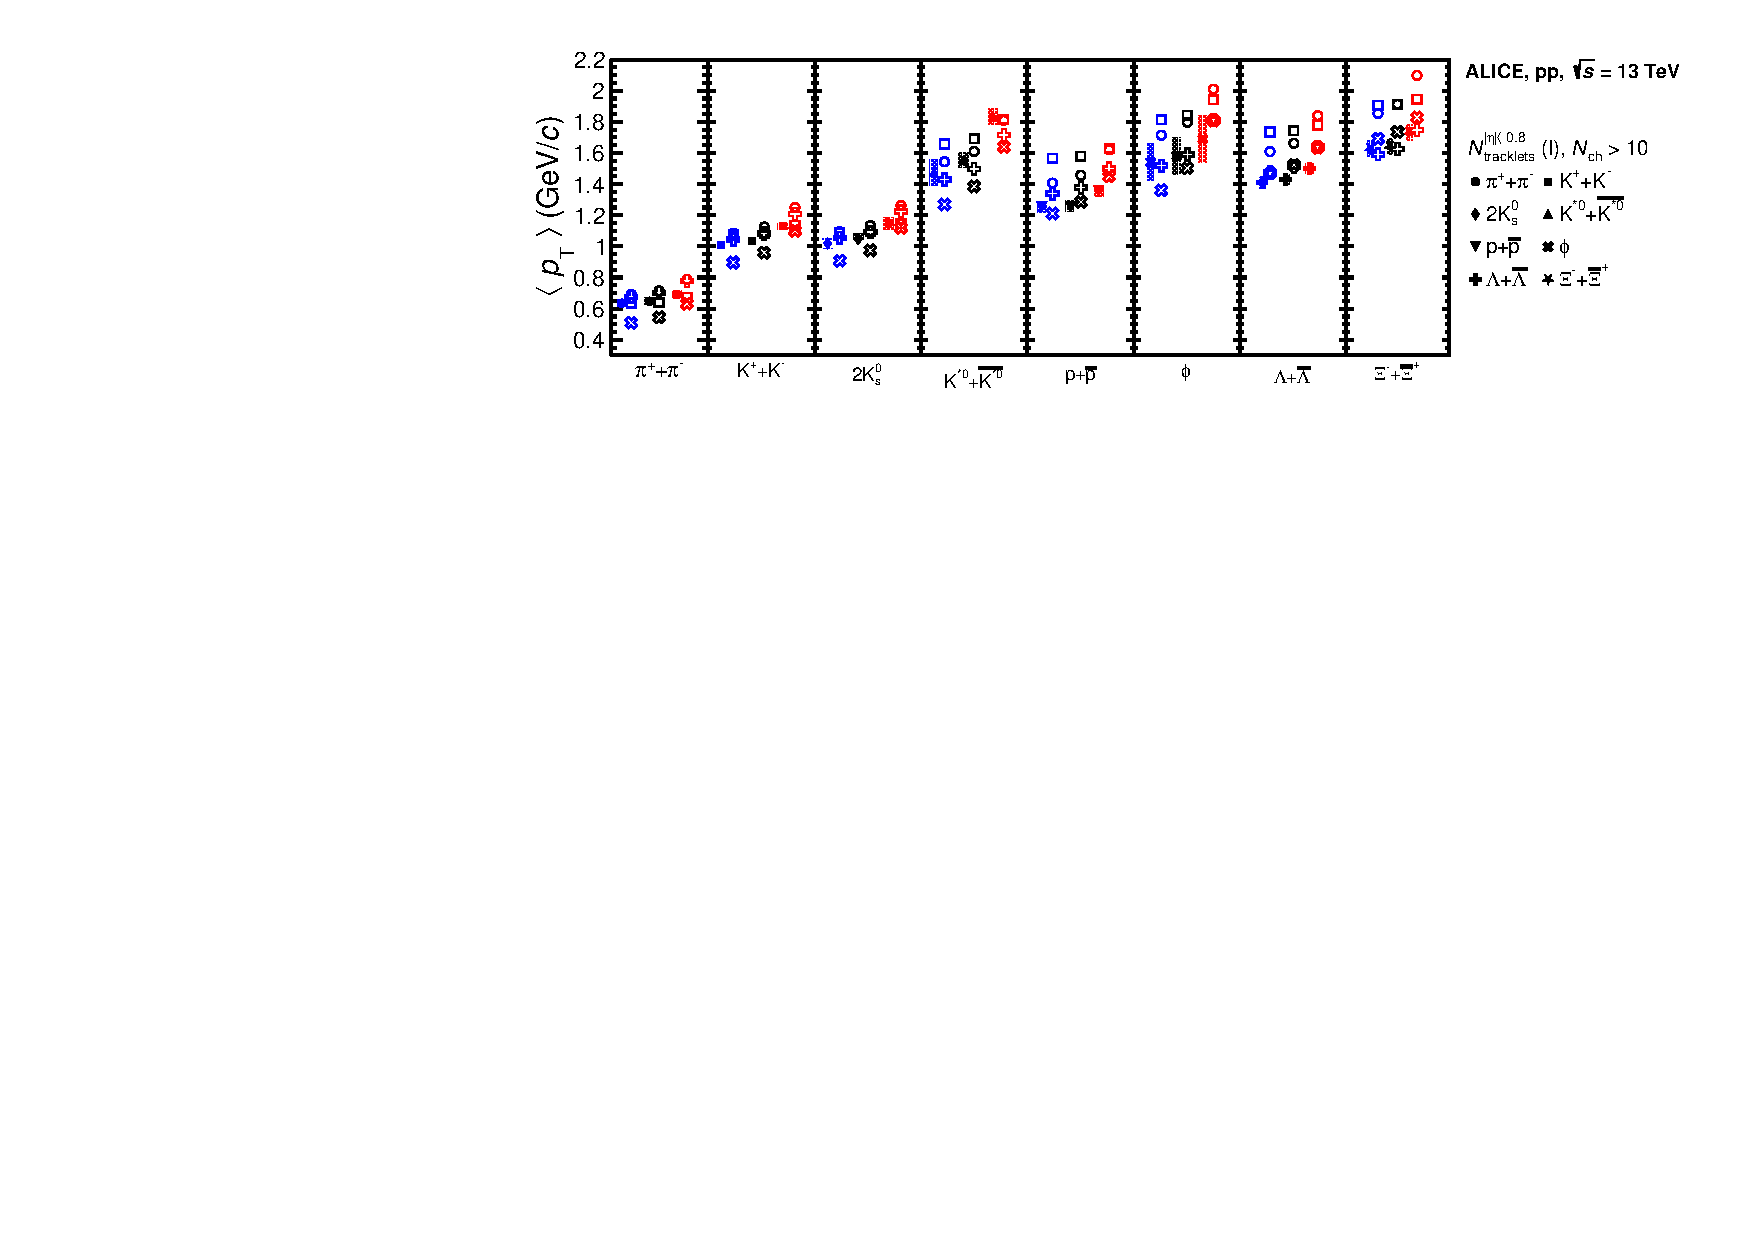
\includegraphics[scale=0.84]{figures/meanPt_0_1_CL1_sp10_pp13_MC_comparisons_2_new.pdf}
    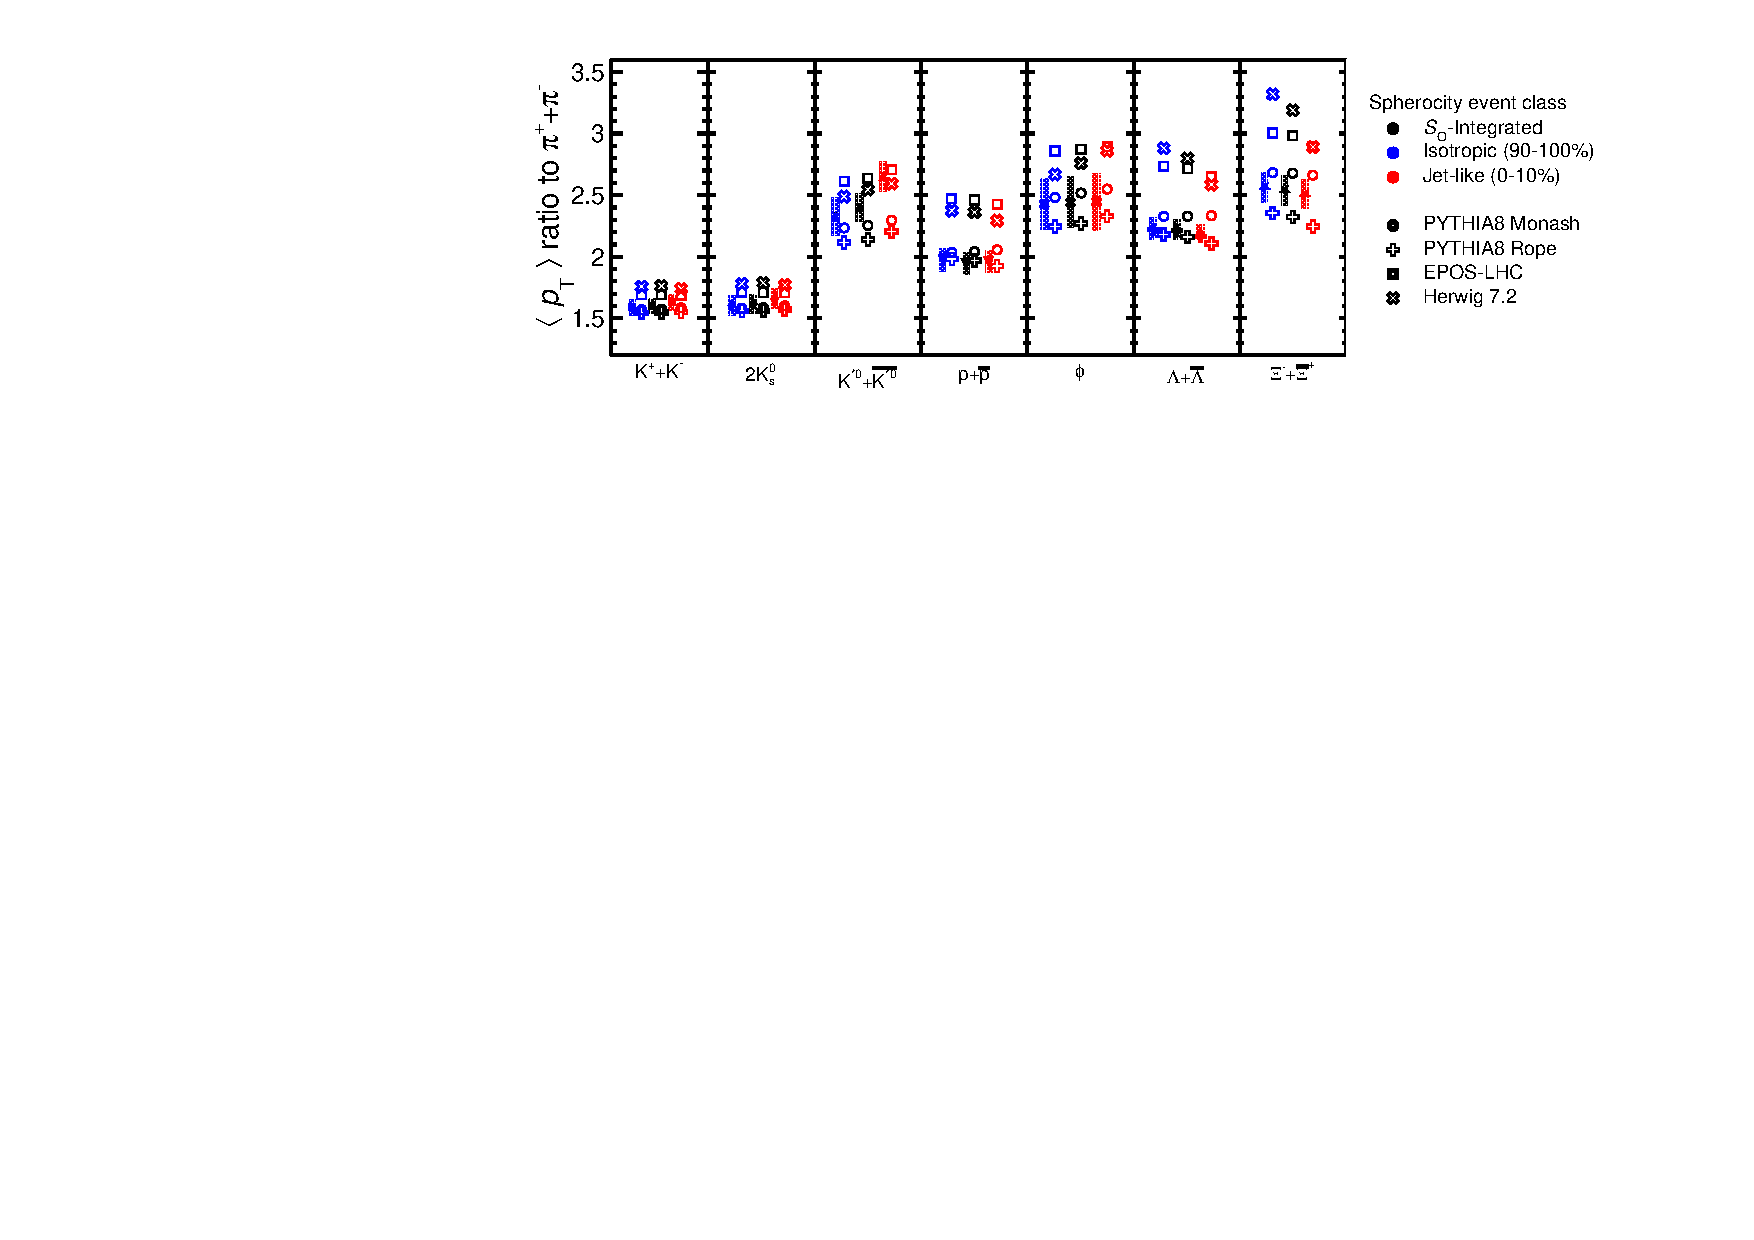
\includegraphics[scale=0.84]{figures/meanPtRatioToPion_0_1_CL1_sp10_pp13_MC_comparisons_2_new.pdf}
    \hspace*{-2.45cm}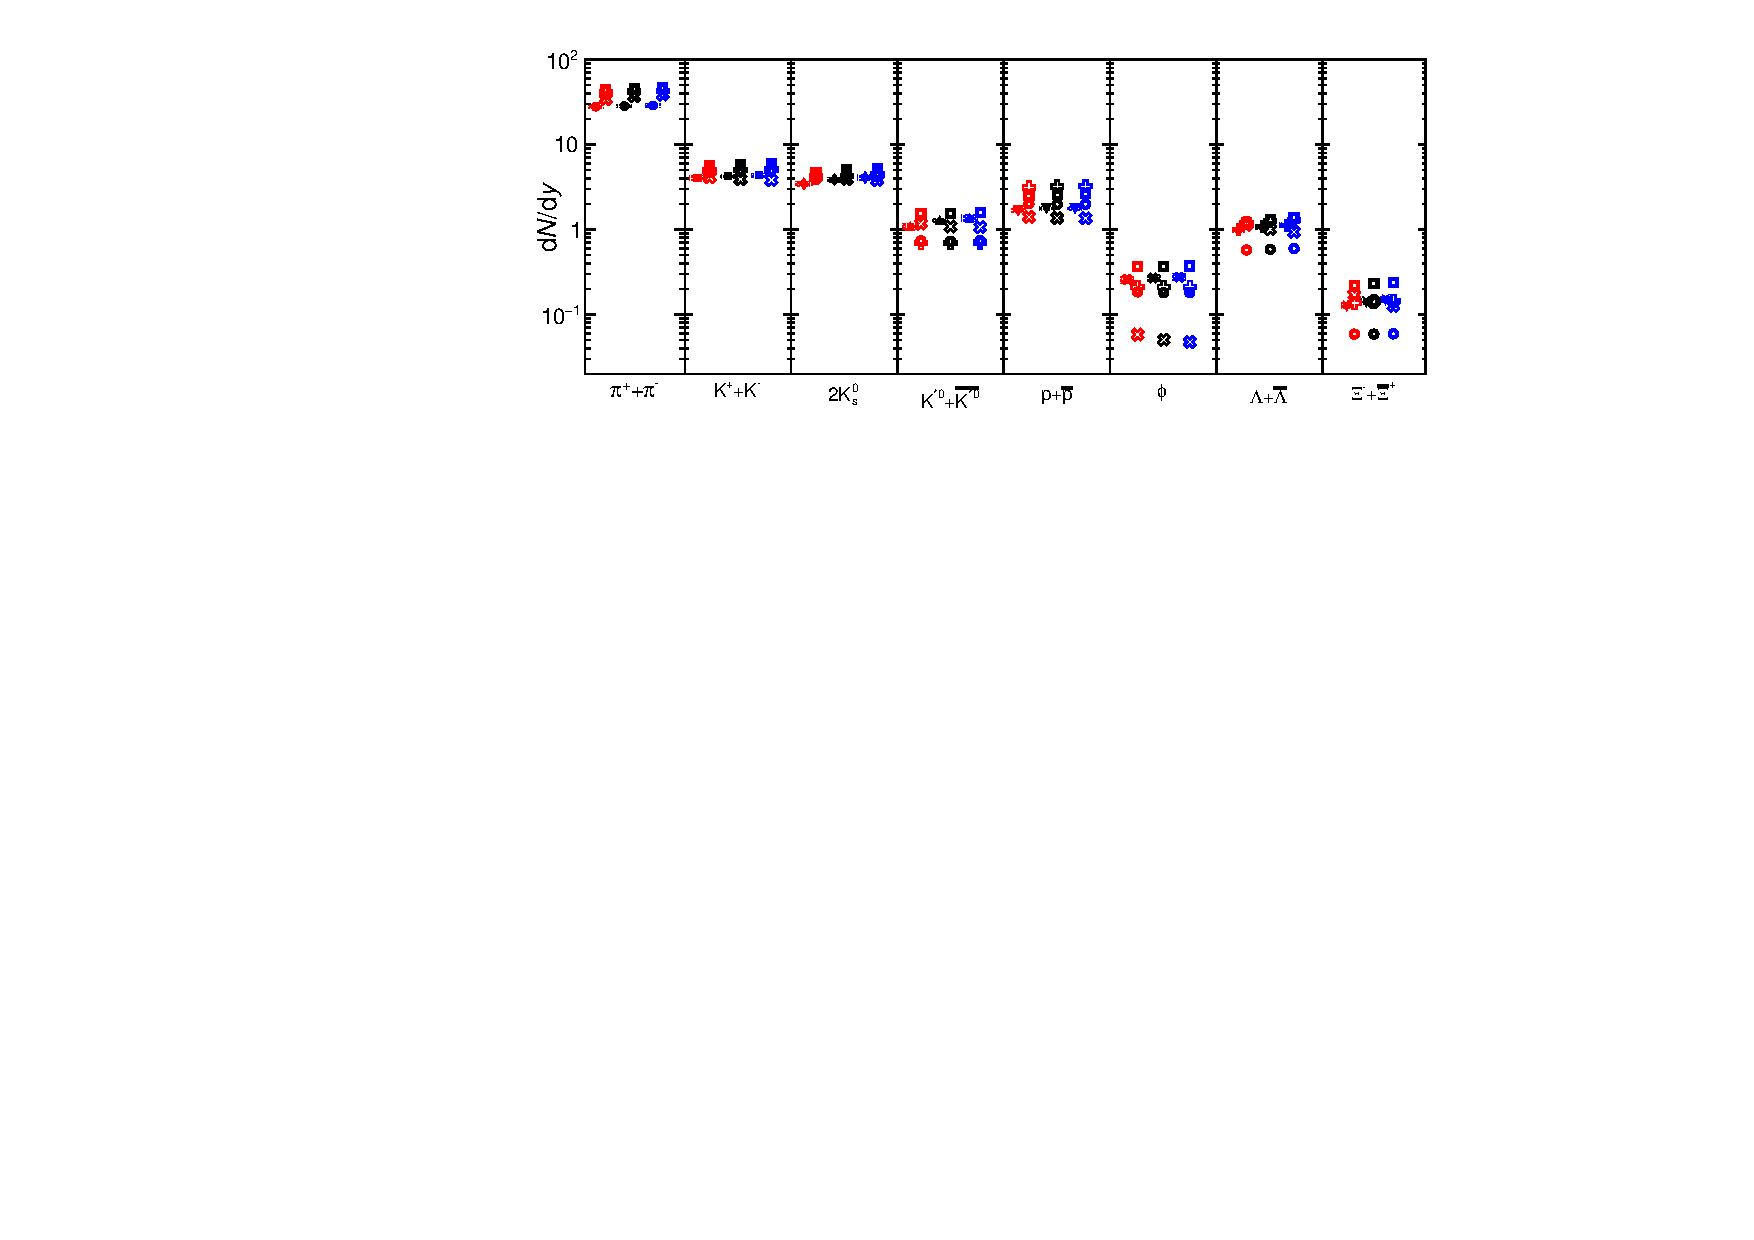
\includegraphics[scale=0.84,trim={0 0 4.6cm 0},clip]{figures/yield_0_1_CL1_sp10_pp13_MC_comparisons_2_new.pdf}
    \hspace*{-1.3cm}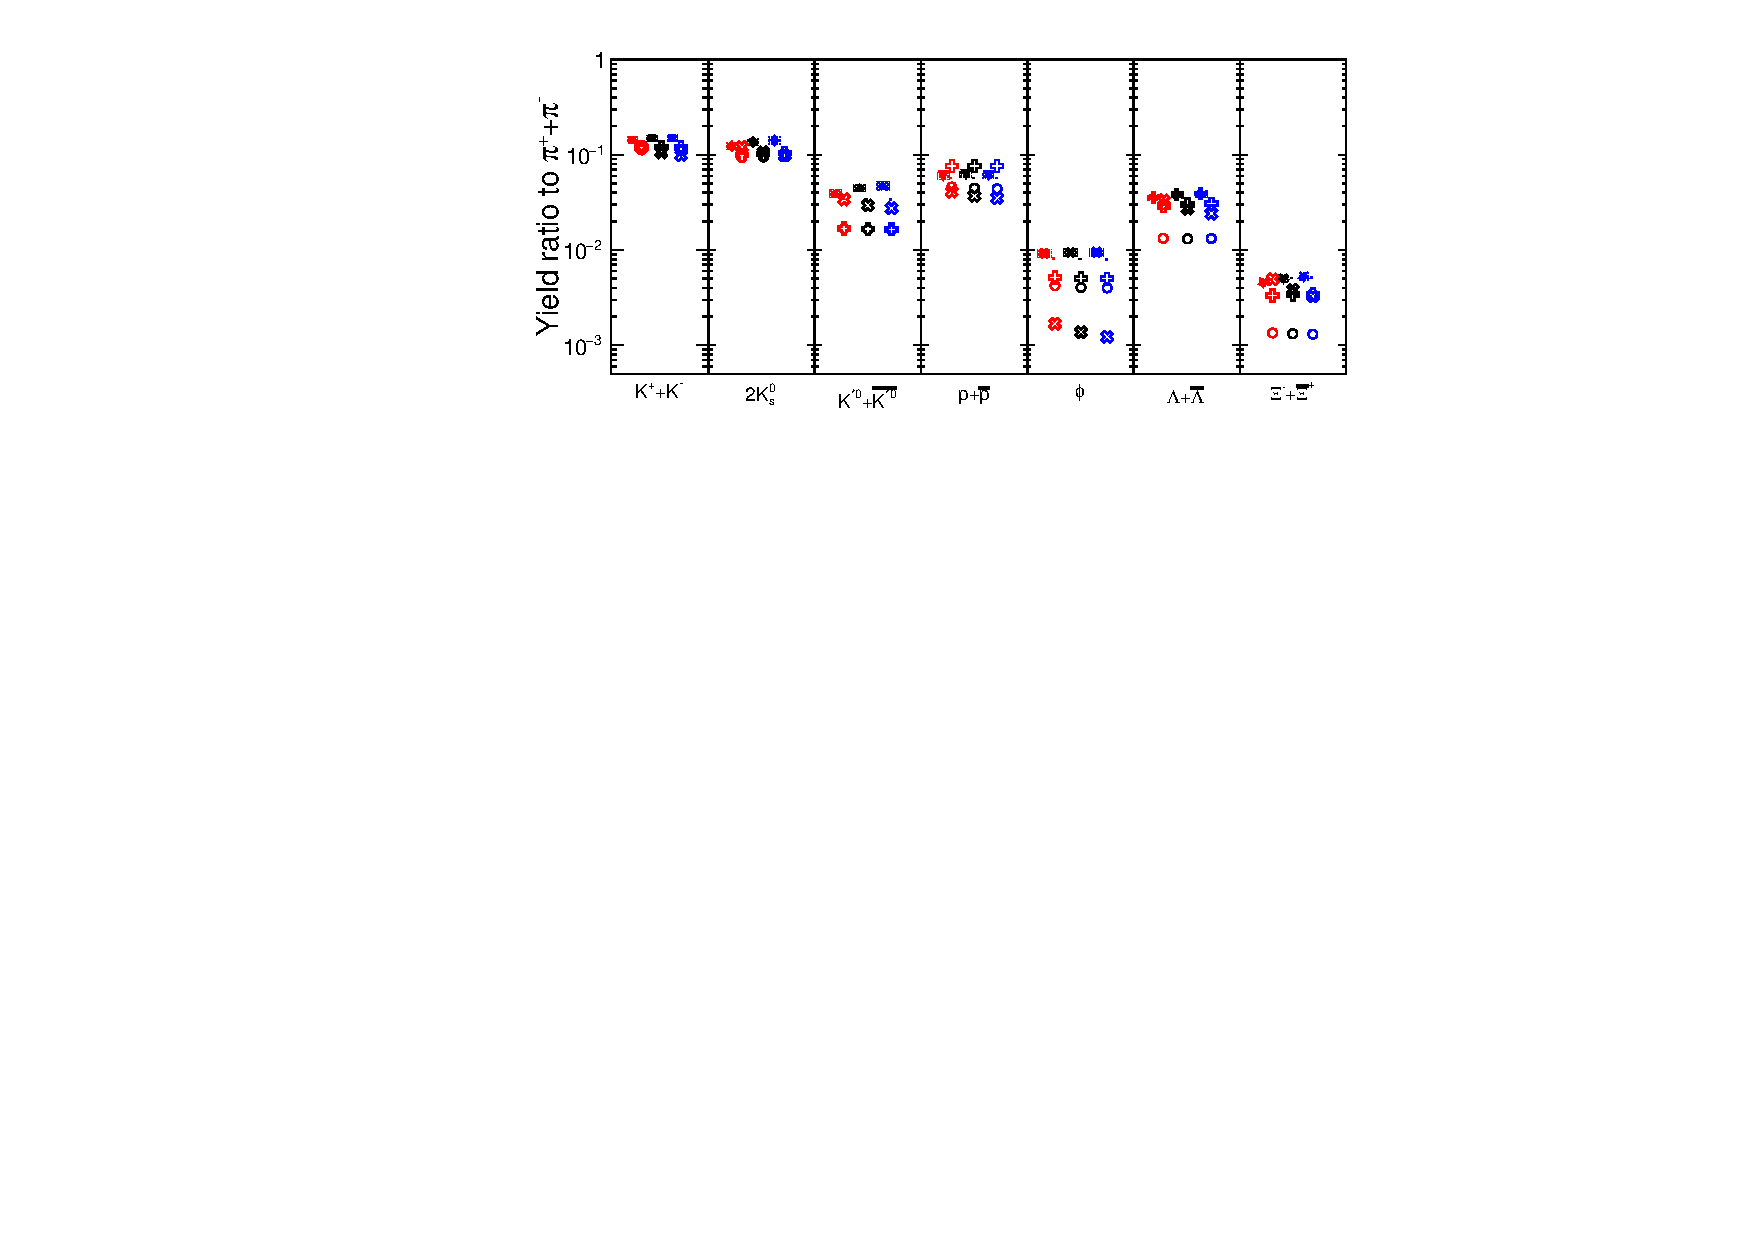
\includegraphics[scale=0.84,trim={0 0 5.9cm 0},clip]{figures/integratedRatioToPion_0_1_CL1_sp10_pp13_MC_comparisons_2_new.pdf}

\caption{The \mpt and \myield  as a function of particle masses obtained for the various particle species in \SOPT classes selected for  high-multiplicity events, determined by the events in the 0--1\% of \tracklet. Upper (lower) panels show the \mpt (\myield). The total systematic uncertainty is represented by the shaded regions. The measured data is compared to predictions from PYTHIA8 Monash, PYTHIA8 Rope, EPOS-LHC, and Herwig 7.2.}
    \label{Fig:Levy}
\end{figure}

 The \SOPT-differential average \pt (\mpt) and yield \myield are reported in Fig.~\ref{Fig:Levy} as a function of the extracted particle masses. The measured \mpt values confirms what is qualitatively observed in the \pt-differential spectra: there is a significant \pt-hardening in jet-like events, and this trend is consistent across all measured light-flavor particle species. Furthermore, the \mpt of the integrated \SOPT high-multiplicity events are consistent with the \mpt of the isotropic sample. This observation indicates that average high-multiplicity events and \SOPT selected isotropic events are dominated by similar underlying physics processes.
 This shows that the \SOPT-integrated event class is not the arithmetic average of the jet-like and isotropic subsamples, indicating that jet-like events are rare outliers of a much more homogeneous group of high-multiplicity events. This observation is of particular interest, and we will focus on exploring it in further detail in the following. 
 
The bottom panels of Fig.~\ref{Fig:Levy} show that the top-1\% \tracklet estimator constrains the variance in \myield between the different \SOPT classes, for all measured particles.  Hence, any observed deviations in comparisons between \tracklet 0--1\% jet-like and isotropic events are unlikely to be driven by a trivial difference in multiplicity. This is not only true for the \PI mesons as reported in Section~\ref{Sec:ResHM}, but across all measured particle masses as a function of \SOPT. 

Most of the presented models overestimate the \mpt for all particle species except \KSTAR, however, this effect can be partially explained by the fact that the models and data are compared at different midrapidity charged particle multiplicities~\cite{ALICE:2020nkc}. Moreover, the models give a reasonable description of the particle specie differences when one normalizes the \mpt relative to that of pions. Furthermore, one can note that the PYTHIA 8.2 predictions, in particular with the enabled color rope framework, overestimates the production of protons and pions, but qualitatively describes the production of most strange hadrons. Moreover, the color rope framework seems to primarily affect the baryons, as the resonance particles show only a small difference in the integrated yield between PYTHIA 8.2 color rope framework and the default PYTHIA 8.2 Monash, in particular for the \KSTAR. In contrast, EPOS-LHC describes the production rates of most particles within the uncertainties of the data, but is unable to capture the trend seen for charged kaons. Herwig 7.2 is unable to capture most of the trends observed in the measured data.

